This chapter first describes the two datasets MS COCO and 3Dshapes used in this work. Then, the agents' architecture is presented. There are two agents---the speaker and the listener agents---whose architectures are shared across all experiments. Finally, the single experiments and their results are discussed.

\section{Datasets}

This work uses two datasets for the reference game. The dataset chosen for the main experiments is the MS COCO Captions dataset \parencite{chen2015microsoft}. As it is one of the most widely used image datasets containing real photos of common objects and scenes, this choice was motivated by the goal of this work is to test multi-agent communication on natural images annotated with natural language captions. 

Further, a second dataset was chosen for conducting baseline experiments in order to investigate potential sources of language drift---the 3Dshapes dataset developed by \textcite{burgess20183d}. This dataset was chosen due to its systematic content and exhaustive annotations of all relevant image features, allowing to automatically generate exhaustive natural language captions for the dataset. This dataset is less noisy and has far less features and categories varying across the images compared to the main dataset, providing a baseline for estimating the models' performance in a more controlled environment.

Both datasets are used for constructing the reference game which procedes in the following way:
\begin{enumerate}
	\item A random image is sampled from the dataset as the target $t$.
	\item A second image is sampled as the distractor $d$ (either at random or following constraints; see below for details).
	\item The speaker agent $S$ recieves both images, the target image being marked respectivaly. It emits a message $m$ describing the target.
	\item The listener agent $L$ recieves both images along with the message $m$, but doesn't know which image is the target.
	\item The listener selects the target image based on the message. If the selection was correct, both agents receive a positive reward, and a negative one otherwise.	 
\end{enumerate}

The next two sections describe in detail the properties of the datasets and how they were preprocessed for the experiments.

\subsection{MS COCO}
The MS COCO Captions dataset \parencite{chen2015microsoft} contains images and respective annotations from the 2014 split of the MS COCO dataset \parencite{lin2014microsoft}. The dataset contains 82,783 images in the training split, each associated with around five human-annoated caption, resulting in a total of 414,113 unique image-caption pairs. The validation split contains 40,504 images, annotated with a total of 202,654 human-produced captions. The respective dataset splits and annotations were downloaded from \url{https://cocodataset.org/#download}.
Furthermore, each image is annotated with bounding boxes of objects and category labels for the depicted objects. There are 80 different basic-level annotation categories, listed in the Appendix \ref{appendix}. These 80 categories are grouped into 12 superordinate categories: person, accessory, indoor, appliance, food, kitchen, sports, furniture, outdoor, animal, electronic and vehicle.
On average, 2.9 basic-level categories and 2.3 superordinate categories occur per image.
\pt{There will be a table with super-basic category mappings and counts of at least each super category}.

The natural language captions associated with the images contain a total of 24,697 unique tokens. Yet over 99\% of the words occuring in the entire dataset are covered by 6000 most frequent tokens. 
The final size of the vocabulary $V$ used in the experiments is 4054, including four special tokens \texttt{START, END, UNK, PAD}, as it comprises over 98\% of the token distribution mass, while comprising 16.4\% of unique tokens occurring in all captions. This vocabulary size was chosen as a good trade-off between a sufficient variety of words that the speaker can choose to describe the images and an action space size which is still learnabale in the current set-up. 

The minimal caption length occuring in the dataset is six tokens, the maximal length is 57 tokens. The mean caption length is 11.3 tokens (based on tokenization with the basic English tokenizer provided by the \texttt{torchtext} package). Since recurrent neural networks may have issues with learning very long sequences \pt{REF}, captions exceeding the length of 15 tokens were truncated. This cut-off length was chosen because it is the minimal length at which over 99\% of the captions didn't have to be truncated. \pt{maybe include a density plot, side by side with the vocab count density one}
During preprocessing, the captions were lowercased, tokenized with the \texttt{torchtext} tokenizer mentioned above and mapped to numerical indices.  The resulting vocabulary is shared between the speaker and listener agents in all experiments. 

For training the agents in the baseline reference game and the fixed-listener experiment, the same 100,000 image-caption pairs sampled at random were used. In this split, there are 61,993 unique images, out of which 33,051 images only occur once. 68 occur five times in the data subset; all other images occur less often. Around 7,000 image-caption pairs from the validation set were used for testing purposes. 
The following preprocessing steps were applied to all images before training: the images were resized to 256 pixels, random $224\times224$ pixel crops were taken, images were horizontally flipped with a probability of 0.5 and each RGB channel was normalized using values expected by the pretrained ResNet50 module (see below for details).

For the baseline experiments, the training pairs of images were sampled at random. In contrast, for the experiment involving similar training pairs the images were sampled such that the distractor depicted objects similar to the target. This was controlled via the category annotations accompanying each image. The training pairs were constructed so that they were annotated with at least three same basic-level categories, or, in case there were less than three, if all annotated categories matched.

\subsection{3Dshapes}
The 3Dshapes dataset introduced by \textcite{burgess20183d} contains 480.000 synthetically generated images. These images depict different three-dimensional geometric objects in abstract space, systematically varying along six different features. These features are the color of the ground on which the object resides (ten values), the color of the background walls (ten values), the color of the object itself (ten values), the type of object (four values), its size (eight values) and its position within the depicted room (15 values). %\pt{Table X depicts / describes the possible values of each dimension}. 
The $64\times64$ pixel images are labeled with six-dimensional vaectors, each position representing the value of one of the six features. 
\pt{Show some examples}.
The dataset was downloaded from \url{https://storage.cloud.google.com/3d-shapes/3dshapes.h5}.
%\pt{XXX images were used for training the agents in the 3Dshapes experiment, and YYY images were used for testing.}

\subsubsection{Caption Generation}
\pt{TBD. Cite Bruni's paper with the grammar stuff.}
%This dataset was chosen due to the systematicity of its content , allowing to generate natural language captions for each image which would exhaustively describe all features of the images. Since no such captions exist to the author's knowldege, they are generated as part of this thesis. To this end, a base context-free grammar (CFG) containing production rules for captions was manually created. The syntactic rules were constructed on the basis of examples of captions created by the author for samples from the dataset. Each caption must contain descriptions of all six feature dimensions. The terminal production rules mapping the pre-terminal to natural language labels are chosen for each image based on its unique feature value configuration. For each image, \pt{X captions are sampled from all the possible productions allowed by the grammar}.

%\pt{Discuss aspects to be taken care of, like vocab size, caption lengths etc}.

\section{Architecture}
The architecture of the agents follows \textcite{lazaridou2020multi}, except minor details to be explained below. \textcite{lazaridou2020multi} explore different ways to parametrize the speaker agent, and the current work replicates the ``multi-task learning'' parametrization (p. 5). This choice is motivated by the fact that among their architectures, this is the only one where the speaker agent learns to produce messages and its core image captioning capability while having access to both the target and the distractors, as opposed to models relying on sampling captions from a pretrained single-image captioning models.\footnote{I think that the multi-task learning set up by \textcite{lazaridou2020multi} really doesn't use pretraining---see their Appendix A ResNet module note.} 

Both agents have two components: a visual embedding module which takes as input the target and distractor images, and a language module. More specifically, the visual module for both agents embeds image features which were extracted using the same pre-trained ResNet50 model \parencite{he2016deep}. The weights were accessed through the \texttt{torchvision.models} API \parencite{marcel2010torchvision}. Features from all training images of the dataset were extracted and saved and then retrieved when training all agents. 
The language module differs for the two agents, so details are provided below. 
The code for all experiments can be found under \url{https://github.com/polina-tsvilodub/mSc-thesis/tree/refGame-noPretrain-token0}. 

\subsection{Speaker}
The speaker receives as input tuples \texttt{(targets, distractors)}, where \texttt{targets} as well as \texttt{distractors} are features extracted from the ResNet50 for the sampled pairs, respectively. That is, the speaker knows which of the the two images in a given iteration of the reference game is the target for which the message should be produced. The speaker then produces a probability distribution over vocabulary tokens of the message given the input $P(m | i_t, i_d)$, parametrized by the speaker model parameters $\theta_S$.

The speaker model consists of a linear layer which projects the 2048-dimensional image features to 512-dimensional embedding space. \pt{Not sure if the dimensionality is also different from what \textcite{lazaridou2020multi} do because of their details in the appendix. Depends on the final way to add visual embeddings to the LSTM and the word embedding dimensions.} The linear layer is first applied to the target images and then to the distractors, resulting in embeddings $i_t$ and $i_d$, respectively. The vectors are concatenated to $[i_t; i_d]$, the target embeddings always being the first ones, such that the speaker network implicitly knows which features represent the target. These 1024-dimensional vectors are used as input to the speaker's language module. The core of the module is the recurrent Long Short-Term Memory (LSTM) cell \parencite{hochreiter1997long}. More specifically, the language module consists of three layers: an embedding layer, mapping the vocabulary to 1024-dimensional word embeddings, a one-layer LSTM with 512-dimensional hidden and cell states; and a linear layer on top, mapping the last hidden state of the LSTM to a score over the vocabulary. The size of the vocabulary depends on the dataset (see above).

During the reference game training, the speaker receives pairs of images, embeds them and passes the concatenated embedding as input to the LSTM. In order to sample the caption for the target, this embedding is prepended to the embedding of the \texttt{START} token. This two-token sequence is then passed to the LSTM and the linear output layer. The next token is sampled from a categorical distribution parametrized with the probabilities computed from the hidden state in the previous timestep, embedded and passed through the LSTM analogously, until the \texttt{END} token is sampled or the maximum caption length is achieved. The design wherein the image embedding is used as the initial token differs from the original design by \textcite{lazaridou2020multi} who prepend the image embedding to each word embedding at each generation time step. This decision had to be made because exploratory experiments showed that the original arcitecture doesn't work for the data at hand.\footnote{\pt{deatils if necessary.}} This is also a common practice in image captioning literature \pt{REF!}. Another possible approach that could be explored in future work would be to initialize the hidden states of the LSTM with the visual embeddings. In this case, the hidden and cell states of the LSTM were initialized with random values sampled from the standard normal distribution.The embedding and last linear layers' weights were initialized with random values sampled from the uniform distribution between -0.1 and 0.1, the biases were initialized with zeroes.  
This architecure results in a total of 10,429,910 trainable parameters.  \pt{Make a graphic of the models and / or the reference game}.

\subsection{Listener}
The listener receives as input the tuples \texttt{(images1, images2, messages)}, the first two inputs being ResNet50 features of the image pairs, input in random order, such that the agent doesn't know which image is the target. The \texttt{message} is the caption produced by the speaker. The listener then produces scores $P(i|m)$ over images identifying which one is the target, parametrized by the listener model parameters $\theta_L$.

The message is passed to the language module which consists of an embedding layer, mapping the vocabulary to 512-dimensional word embeddings, and a one-layer LSTM with 512-dimensional hidden and cell states. All weights are initialized analagously to the respective weights of the speaker model. The hidden cell state $h_i$ at the last time step of embedding the received message is used as the final message representation. 
The visual module of the listener consists of a linear layer which also projects the 2048-dimensional image features to a 512-dimensional embedding space. The images are passed through the linear layer one after the other, resulting in embeddings $i_1$ and $i_2$. \pt{Unsure about this step, although it follows some implementations of \textcite{lazaridou2016multi} of an analogous step.} Finally, the listener computes the dot products between each image embedding and the message embedding. The target is sampled from a categorical distribution parametrized with probabilities computed based on the dot products.  
The architecture results in 1,049,088 trainable parameters for the listener's visual module and 4,176,896 trainable parameters for its LSTM.

The next section describes how these agents were trained in the reference game setting.

\pt{Circle back to chapter 2 by talking about speaker and listener policies.}

\subsection{General Training Details}

All experiments were trained with a batch size of 64 pairs, using the Adam optimizer with a learning rate  of 0.001 \parencite{kingma2014adam}. In the reference game setting, the models were trained for \pt{X epochs}. 
The speaker parameters $\theta_S$ were updated by optimizing a compound loss function $J_s$. More precisely, the speaker loss consisted of a weighted sum of a functional loss $L_f$ and a structural loss $L_s$. The former was computed via the REINFORCE rule based on the listener's task performance (i.e., referential success). The speaker received the reward 1 if the listener guessed the target successfully, and -1 otherwise. The latter was computed via cross-entropy between the message produced by the speaker and the ground truth caption for the given target image. $L_f$ additionally included an entropy regularization term, weighted by 0.1 \pt{references}. The resulting loss is $J_s = L_f + 0.1 L_s$. 
The listener parameters $\theta_L$ were updated via cross-entropy loss $J_l$ optimized based on the guessed target classification of the images and the ground truth targets. 

\section{Experiments}

\pt{when discussing results and esp PPL, \cite{havrylov2017emergence} also compute encoder PPLs}

\subsection{Speaker Pretraining}
As described in Section \ref{model_pretraining}, there are different strategies for pretraining the speaker. Based on initial exploratory experiments reported in Appendex \ref{app:grid_search}, all speakers were pretrained using an exponentially decreasing teacher-forcing rate $0.5^{epoch-1}$.

\begin{figure}
	\centering
	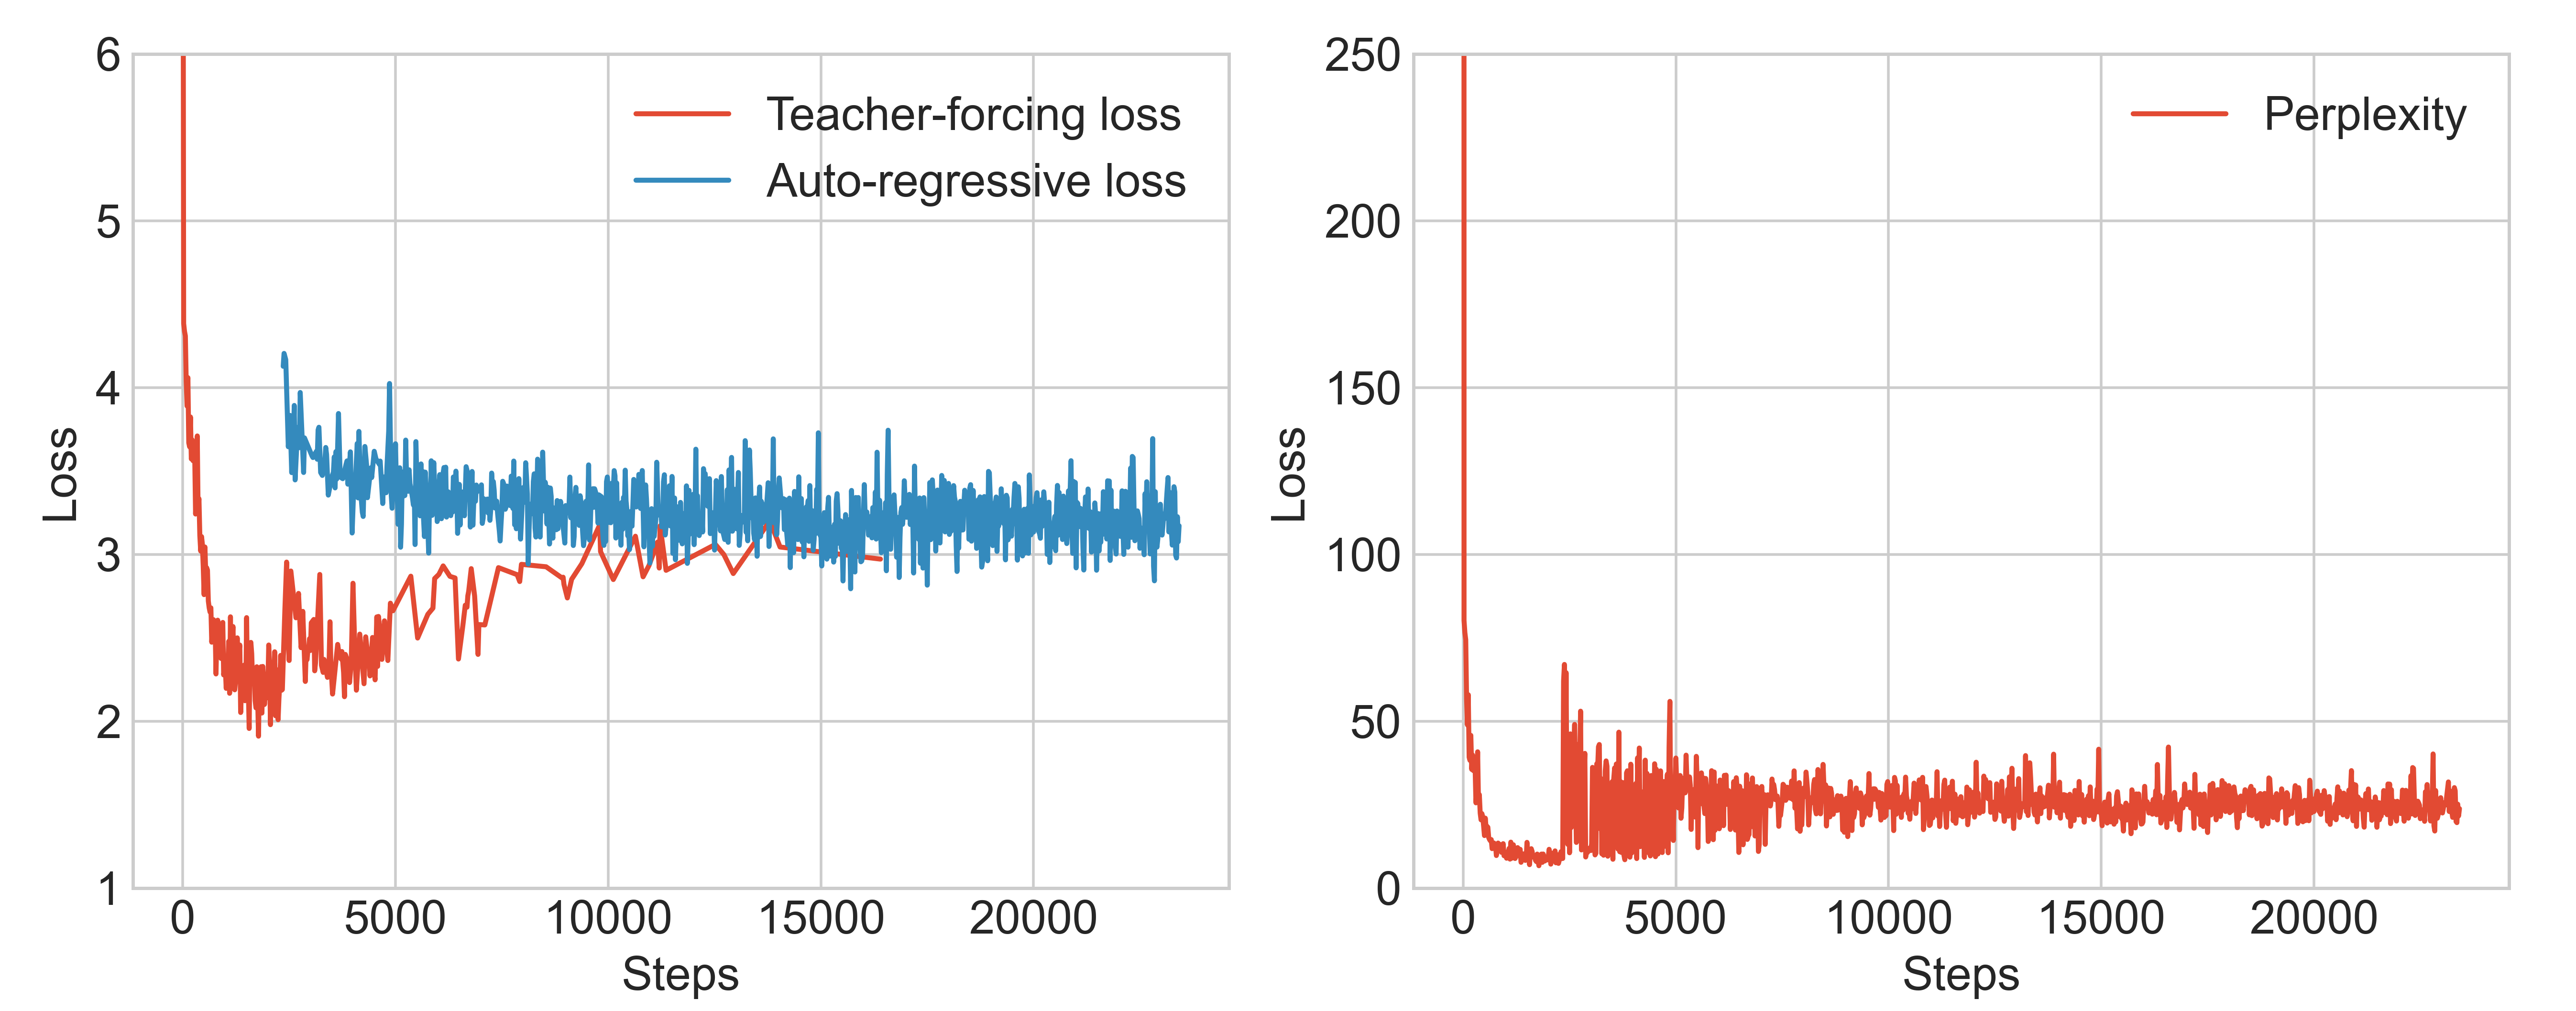
\includegraphics[width=\linewidth]{images/coco_pretraining_losses_ppls.png}
	\caption{A: LSTM cell architecture. B: Image captioner architecture consisting of a CNN image vector extractor (leftmost box) which passes an image vector into an LSTM cell (represented unrolled in time) as initialization of its hidden state.}
	\label{fig:coco_pretraining}
\end{figure}  

%\subsubsection{Training}
%\subsubsection{Results}

%\subsection{Similar Pairs}

%Describe details on training pair generation here. Mention Xenia's recent paper.

%\subsection{3Dshapes Experiment}

%\subsection{Fixed Listener Experiment}